\clearpage

\section{Návod k obsluze zařízení}
\indent\indent Ovládání zařízení je velice intuitivní. Zařízení stačí připojit kabelem, které má na obou koncích konektor stereo Jack 3,5 samec do SDR přijímače na čelní panel a druhý konec do linkového vstupu zvukové karty. Čím bude mít zvuková karta vyšší vzorkovací frekvenci, tím větší pásmo budeme moci sledovat na osobním počítači s obslužným softwarem. Po připojení kabelu stačí k zařízení zezadu připojit napájecí kabel, jedná se o klasickou ,,euro šňůru''. Poté již jen stačí na  čelním panelu stisknout vypínač a na osobním počítači spustit obslužný software Sharp SDR. Ovládání Software je velmi jednoduché. Vlevo na postranním panelu se nastavují parametry zpracování signálu jako: způsob demodulace, šířka pásma, potlačení stejnosměrné složky, potlačení šumu atd. SDR přijímač se ovládá ještě jednodušeji. Otáčením rotačního enkodéru měníme výstupní frekvenci. Pokud stiskneme enkodér, přepneme se do módu, ve kterém otáčením enkodéru měníme ladící krok. Opětovným stiskem enkodéru se dostaneme zpátky do módu ladění přijímané frekvence.

% os b
\begin{figure}[H]
	\centering
	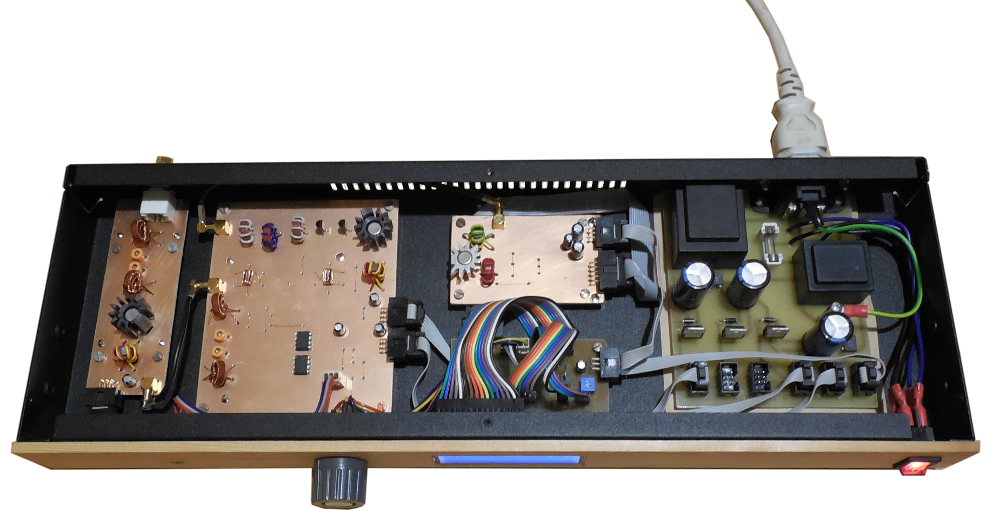
\includegraphics[width=170mm]{img/bez_kritu_sm.png}
	\caption{Hotové zařízení bez horní části krabice}    		
\end{figure}

% os b
\begin{figure}[H]
	\centering
	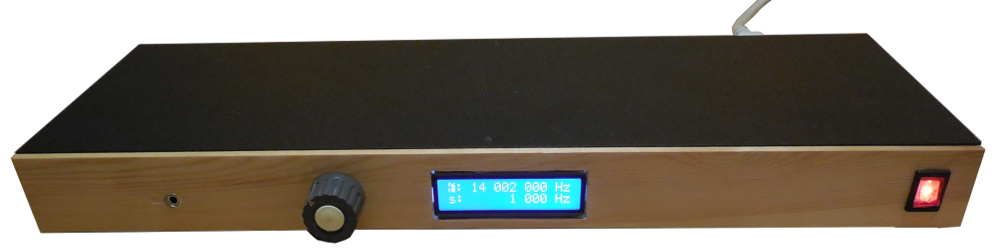
\includegraphics[width=170mm]{img/s_kritem_sm.png}
	\caption{Hotové zařízení v kompletní krabici rackových rozměrů}    		
\end{figure}

\clearpage